\documentclass[12pt,a4paper]{article}

% == FOR DOC AND TESTS - START == %

\usepackage[utf8]{inputenc}
\usepackage{ucs}
\usepackage[top=2cm, bottom=2cm, left=1.5cm, right=1.5cm]{geometry}

\usepackage[francais]{babel}

\usepackage{color}
\usepackage{hyperref}
\hypersetup{
    colorlinks,
    citecolor=black,
    filecolor=black,
    linkcolor=black,
    urlcolor=black
}

\usepackage{multicol}
\usepackage{enumitem}

\usepackage{amsthm}

\usepackage{tcolorbox}
\tcbuselibrary{listingsutf8}

\usepackage{pgffor}
\usepackage{xstring}


% MISC

\tcbset{%
	sharp corners,%
	left=1mm, right=1mm,%
	bottom=1mm, top=1mm,%
	colupper=red!75!blue% 
}

\setlength{\parindent}{0cm}

\theoremstyle{definition}
\newtheorem*{remark}{Remarque}

\usepackage[raggedright]{titlesec}

\titleformat{\paragraph}[hang]{\normalfont\normalsize\bfseries}{\theparagraph}{1em}{}
\titlespacing*{\paragraph}{0pt}{3.25ex plus 1ex minus .2ex}{0.5em}

\makeatother
	\newcommand\resetallcnt{
		\setcounter{lyxam@counter@topic}{0}
		\setcounter{lyxam@counter@exercise}{0}
		\setcounter{lyxam@counter@problem}{0}
		\setcounter{lyxam@counter@bonus}{0}
		\setcounter{lyxam@counter@subpart}{0}
	}
\makeatletter

% Technical IDs

\newwrite\tempfile

\immediate\openout\tempfile=x-\jobname.macros-x.txt

\AtEndDocument{\immediate\closeout\tempfile}

\newcommand\IDconstant[1]{%
    \immediate\write\tempfile{constant@#1}%
}

\makeatletter
	\newcommand\IDmacro{\@ifstar{\@IDmacroStar}{\@IDmacroNoStar}}
	
    \newcommand\@IDmacroNoStar[3]{%
        \texttt{%
        	\textbackslash#1%
        	\IfStrEq{#2}{0}{}{%
        		\,\,[#2 Option%
				\IfStrEq{#2}{1}{}{s}]%
			}%
    	    \IfStrEq{#3}{}{}{%
	    		\,\,(#3 Argument%
				\IfStrEq{#3}{1}{}{s})%
			}
	   	}
        \immediate\write\tempfile{macro@#1@#2@#3}%
    }

    \newcommand\@IDmacroStar[2]{%
        \@IDmacroNoStar{#1}{0}{#2}%
    }

	\newcommand\@IDoptarg{\@ifstar{\@IDoptargStar}{\@IDoptargNoStar}}
	
	\newcommand\@IDoptargStar[2]{%
    	\vspace{0.5em}
		--- \texttt{#1%
			\IfStrEq{#2}{}{:}{\,#2:}%
		}%
	}

	\newcommand\@IDoptargNoStar[2]{%
    	\IfStrEq{#2}{}{%
			\@IDoptargStar{#1}{}%
		}{%
			\@IDoptargStar{#1}{\##2}%
		}%
	}

	\newcommand\IDkey[1]{%
    	\@IDoptarg*{Option}{{\itshape "#1"}}%
	}

	\newcommand\IDoption[1]{%
    	\@IDoptarg{Option}{#1}%
	}

	\newcommand\IDarg[1]{%
    	\@IDoptarg{Argument}{#1}%
	}
\makeatother

% == FOR DOC AND TESTS - END == %


\begin{document}

\section{Quel devoir donnez-vous ?}

	\subsection{La commande \texttt{\textbackslash exam}}

La commande \verb+\exam+ est la commande à tout faire, ou presque, du package \verb+lyxam+.
Elle doit être au tout début du contenu, et elle ne peut être utilisée qu'une seule fois.


\medskip


Le code ci-dessous donne tous les options disponibles où il est important de savoir que seul le paramètre \verb+kind+ est obligatoire.

\begin{tcblisting}{listing only}
\exam[%
    kind      = D.S.,%
    render    = yes,%
    nb        = 1,%
    subnb     = Sujet A,%
    subject   = Mathématiques,%
    theme     = Probabilités \& Fonctions,%
    sector    = Série Scientifique,%
    class     = 1S4,%
    location  = Lycée MONGE (Chambéry),%
    date      = 20/10/2017,%
    time      = 2h,%
    preambule = Ne pas oublier de réfléchir dans ce devoir !%
]
\end{tcblisting}


\newpage


Vous obtiendrez alors une mise en page du type suivant où pas mal de choses sont gérées pour vous.

\begin{center}
	\begin{multicols}{2}
		\setlength{\fboxsep}{5pt}
		\setlength{\fboxrule}{1pt}

		\fbox{
\includegraphics[width=0.9\linewidth]{example-doc[fr]-0.jpg}}

		\fbox{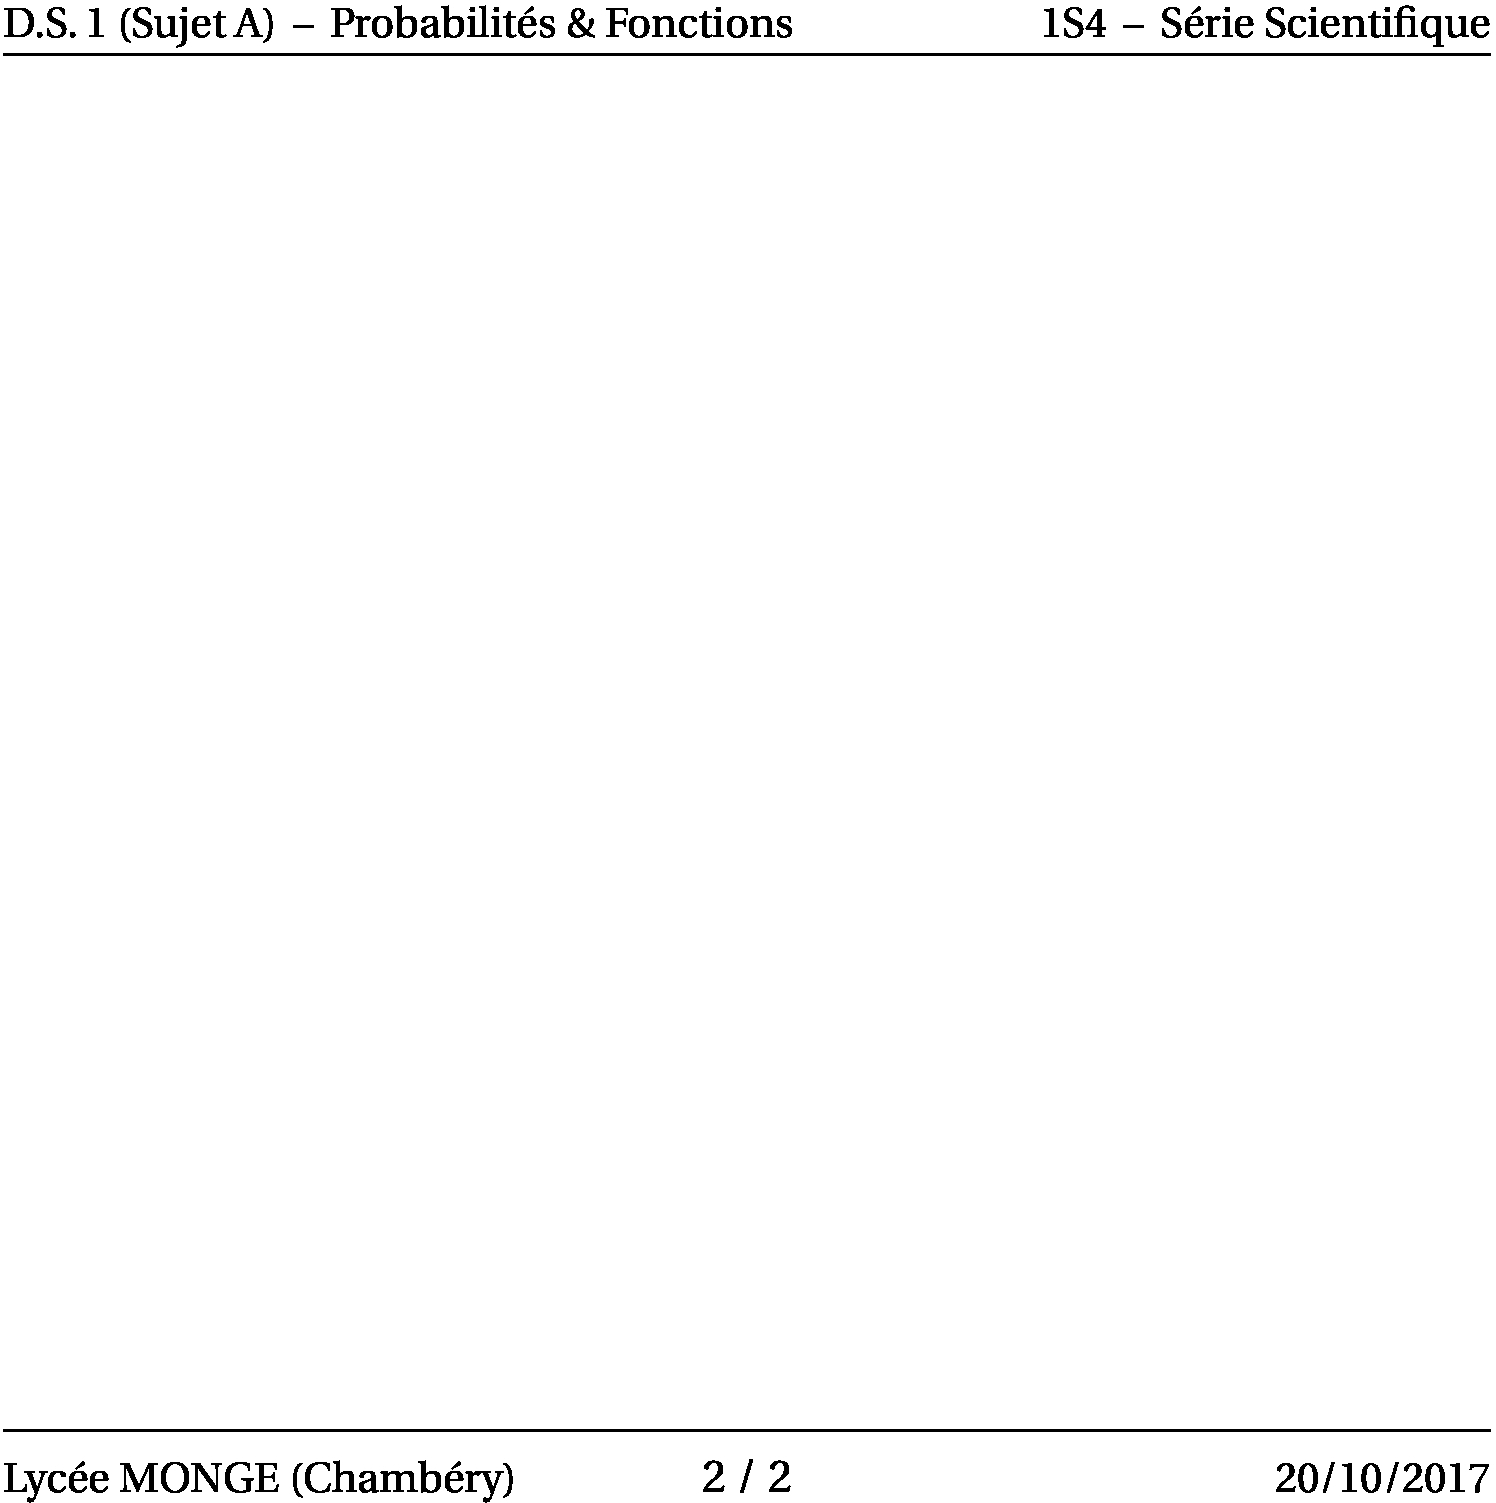
\includegraphics[width=0.9\linewidth]{example-doc[fr]-1.jpg}}
	\end{multicols}
\end{center}


Expliquons en détail le rôle de chacun des paramètres qui ont tous des valeurs de type texte \emph{(comme c'est toujours le cas, ou presque, avec \LaTeX{})}.

\begin{enumerate}
	\item \verb+kind+, \emph{qui doit obligatoirement être renseigné}, est tout simplement le type de devoir : un \emph{"D.S."}, un \emph{"D.M."}, une \emph{"Interrogation Surprise"}, une \emph{"Fiche d'entraînement"}, une \emph{"Activité"}...
	Vous noterez que le terme \emph{"devoir"} ne se limite pas juste aux devoirs notés.

	\item \verb+render+ est à utiliser pour un sujet à rendre avec la copie : utiliser \verb+yes+ ou \verb+no+ pour \emph{"oui"} ou \emph{"non"}.
	Ceci a pour conséquence que le sujet débutera, ou non, par une zone où l'élève devra indiquer son nom et son prénom.

	\item \verb+nb+ porte bien son nom : c'est le numéro du devoir.

	\item \verb+subnb+ permet d'indiquer une sorte de numérotation secondaire. C'est utile par exemple pour indiquer \emph{"Sujet A"}, \emph{"Sujet B"} ...

	\item \verb+subject+ permet si besoin de donner la thématique générale du devoir comme par exemple \emph{"Mathématiques"}, \emph{"Informatique Générale"}...

	\item \verb+theme+ sert à compléter la thématique générale en indiquant un ou des points particuliers comme par exemple \emph{"Probabilités"}, \emph{"Réseaux"} ...

	\item \verb+sector+ sert à indiquer une section, au sens administratif, à laquelle s'adresse le devoir. Par exemple, pour un sujet de Bac S en France, on utiliserait \verb+sector = Série Scientifique+.

	\item \verb+class+ indique la classe et/ou le groupe auquel est destiné le devoir.

	\item \verb+location+ vous permet d'indiquer un lieu géographique, typiquement un établissement scolaire ou universitaire.

	\item \verb+date+ est pour la date du devoir.

	\item \verb+time+ est pour la durée du devoir.

	\item \verb+preambule+ vous aidera à indiquer un texte en préambule qui apparaîtra avant vos exercices pour par exemple rappeler des obligations légales ou bien des choses importantes.
	 Si vous avez besoin de faire des retours à la ligne dans votre préambule, vous avez deux possibilités :

	 \begin{enumerate}
		\item Le mieux est de définir une macro commande où vous taperez votre texte.

		\item Si vous ne savez pas comment créer une macro commande, vous pouvez simplement utiliser des accolades et \verb+\\+ pour chaque retour à la ligne comme par exemple dans \verb+preambule = {Ligne 1\\Ligne 2\\Ligne 3}+.
	\end{enumerate}
\end{enumerate}


	\subsection{Différentes mises en forme}

Le package est fourni avec des exemples de fichiers \LaTeX{} afin d'observer ce que permet \verb+lyxam+. Explorez-les !


	\subsection{Fiche technique}

\IDmacro{exam}{12}{0}

\IDkey{kind} le type de devoir. \emph{Ceci ne peut pas être un texte vide.}

\IDkey{render} pour un sujet à rendre, ou non, avec une zone pour le nom et le prénom de l'étudiant. Deux valeurs possibles : \verb+yes+ ou \verb+no+ (valeur par défaut).

\IDkey{nb} le numéro du devoir.

\IDkey{subnb} une numérotation secondaire du devoir.

\IDkey{subject} la matière, le sujet du devoir.

\IDkey{theme} un sous-thème ou une sous-partie de la matière ou du sujet du devoir.

\IDkey{sector} un secteur, une section, au sens administratif, à laquelle s'adresse le devoir.

\IDkey{class} la classe concernée par le devoir.

\IDkey{location} le lieu géographique où a lieu le devoir.

\IDkey{date} le texte donnant la date du devoir.

\IDkey{time} le texte indiquant juste la durée du devoir.

\IDkey{preambule} un texte en préambule du devoir pour rappeler des obligations légales ou bien des choses importantes.

\end{document}
